\chapter{Introdução a Redes Neurais}
\label{ch:03}


% \epigraph{\itshape Those who cannot remember the past are condemned to compute it.''}{---Steven Pinker, \textit{Words and Rules}}

\section{Redes Neurais}

Uma rede neural é, essencialmente, um modelo de aprendizado de máquina supervisionado %[ref] 
que está a procura de aprender \textit{padrões}. Um modelo de aprendizado de máquina é uma tarefa computacional que explora algoritmos que podem aprender a partir de seus erros e fazer previsões sobre dados. A principal característica desse tipo de modelo é o caráter indutivo dos algoritmos, em oposição aos dedutivos. Esse tipo de algoritmo é normalmente inicializado com nenhuma expectativa sobre a tarefa que deve realizar e busca informações exclusivamente a partir dos dados do problema. Os possíveis tipos de aprendizado de máquina são divididos entre: \textit{supervisionados}, \textit{não-supervisionados} %ref
e por \textit{reforço}. %ref
No caso das redes neurais, o aprendizado diz-se supervisionado, pois informa-se à rede o \textit{output} esperado pelo treinamento.

A inspiração para o desenvolvimento da modelagem em redes neurais aritificiais surgiu a partir de estudos em neurosciência %[ref] 
que concluiram que, diante de múltiplas apresentações de um mesmo estímulo, um mesmo grupo de neurônios sofre incitação e dispara (\cite{hubel:1962}).  Analogamente, o modelo artificial é composto por uma camada de \textit{input} que recebe diferentes estímulos (vetores numéricos que representam o objeto a ser analisado). A informação recebida é distribuída ao longo de múltiplas conexões com a próxima camada através de uma múltiplicação com uma matriz de pesos $\vect{W}$. A matriz de pesos funciona como uma analogia às conexões existentes entre neurônios de modo que um peso maior representa uma conexão que deve ser reforçada e um peso menor representa uma conexão que deve ser reprimida. Além disso, é importante que o sistema de aprendizado não seja demasiado sensível a todo \textit{input} que receber, pois nesse caso cada \textit{input} diferente recebido alteraria completamente o modelo impossibilitando um aprendizado generalizado. Como solução, o resultado obtido a partir da multiplicação dos pesos pelos \textit{inputs} entra como argumento em uma função de ativação. A função de ativação é uma função que simula o potencial energético existente entre as conexões neurais e permite que uma unidade apenas seja ativada caso o resultado dessa função atinja um \textit{threshold} mínimo. Isso permite ao sistema a produção de diferentes respostas para padrões diferentes utilizando a mesma rede e além disso, permite que o aprendizado ocorra de forma gradual, de modo que o efeito de estímulos passados ainda perdure por um longo período mesmo após a apresentação de novos estímulos. Uma das funções de ativação mais utilizadas na literatura (e inclusive utilizada pelos pesquisadores Rumelhart e McClelland) é a função \textit{Sigmoid}, uma função suave, diferenciável e facilmente interpretável. A Fig. \ref{fig:sigmoidplot} ilustra o processo de ativação dado um \textit{input} $\vect{x}$. Supõe-se que um neurônio seja ativado apenas se houver uma energia mínima para tal. Da mesma forma, representa-se uma ativação no eixo \textit{y} (com valores entre 0 (não ativação) e 1 (ativação)) de modo que apenas valores mais altos de $\vect{x}$ atingem valores próximos da ativação em \textit{y}.

\begin{figure}[H]
\centering
\scalebox{0.9}{
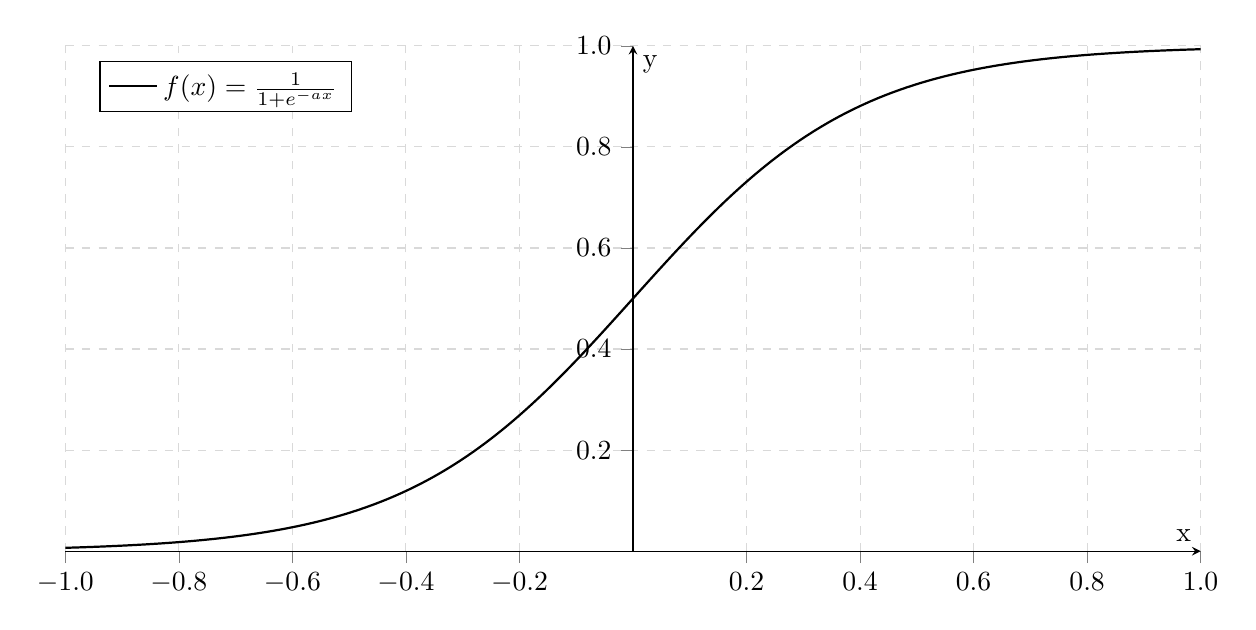
\begin{tikzpicture}
    \begin{axis}[
    	legend pos=north west,
        axis x line=middle,
        axis y line=middle,
        x tick label style={/pgf/number format/fixed,
                            /pgf/number format/fixed zerofill,
                            /pgf/number format/precision=1},
        y tick label style={/pgf/number format/fixed,
                            /pgf/number format/fixed zerofill,
                            /pgf/number format/precision=1},
        grid = major,
        width=16cm,
        height=8cm,
        grid style={dashed, gray!30},
        xmin=-1,     % start the diagram at this x-coordinate
        xmax= 1,    % end   the diagram at this x-coordinate
        ymin= 0,     % start the diagram at this y-coordinate
        ymax= 1,   % end   the diagram at this y-coordinate
        %axis background/.style={fill=white},
        xlabel=x,
        ylabel=y,
        tick align=outside,
        enlargelimits=false]
      % plot the stirling-formulae
      \addplot[domain=-1:1, black, thick,samples=500] {1/(1+exp(-5*x))};
      %\addplot[domain=-1:1, blue, ultra thick,samples=500] {1/(1+exp(-10*x))};
      \addlegendentry{$f(x)=\frac{1}{1+e^{-ax}}$}
      %\addlegendentry{$g(x)=\frac{1}{1+e^{-10x}}$}
    \end{axis} 
\end{tikzpicture}
}
\caption{A função \textit{Sigmoid}.}
\label{fig:sigmoidplot}
\end{figure} %diminuir esse desenho

Após essa passagem pela função de ativação, o resultado serve como novo input para a próxima camada e assim sucessivamente até a última, a camada de \textit{output}. Todas as camadas existentes entre as camadas de \textit{input} e de \textit{output} são chamadas de \textit{camadas escondidas} (Ver Fig. \ref{fig:ffd}.)

% \begin{align}\label{eq:sigmoid}
% p(w_{i} = 1) = \frac{1}{1+e^{\sum_{i} w_{i}x_{i}}}
% \end{align}

Algebricamente, pode-se representar o processo descrito através da composição de múltiplas funções, uma vez que o resultado das operações precedentes servirão como entrada para as próximas camadas.

\begin{align}
% f(\vect{x}) &= f^{(2)}(f^{(1)}(\vect{x}; \vect{W}_1); \vect{W}_2)\\
% &= 
\sigma(\vect{W}_2 (\sigma(\vect{W}_1\vect{x})))
\end{align}

\input{definitions/colors}
\input{definitions/styles}
\begin{figure}[ht!]
\centering

\scalebox{1.0}{
\begin{tikzpicture}[auto]

% operations =========

% FNN input
\node[normal] (x1) {};
\node[textonly, above=10pt of x1] (input) {Camada de \textit{inputs}};
\node[normal, below=10pt of x1] (x2) {};
\node[normal, below=10pt of x2] (x3) {};
\node[normal, below=10pt of x3] (x4) {};
\node[normal, below=10pt of x4] (x5) {};
\node[normal, below=10pt of x5] (x6) {};

% FNN output
\node[textonly, right=50pt of x1] (center) {Camada Escondida};
\node[normal, below=25pt of center] (y1) {};
\node[normal, below=10pt of y1] (y2) {};
\node[normal, below=10pt of y2] (y3) {};

% FNN output
\node[textonly, right=110pt of input] (output) {Camada de \textit{outputs}};
\node[normal, below=15pt of output] (z1) {};

\node[normal, below=10pt of z1] (z2) {};
\node[normal, below=10pt of z2] (z3) {};
\node[normal, below=10pt of z3] (z4) {};
\node[normal, below=10pt of z4] (z5) {};
\node[normal, below=10pt of z5] (z6) {};

% phon features 2

% edges FNN
\path[nedge] (x1) -- (y1);
\path[nedge] (x1) -- (y2);
\path[nedge] (x1) -- (y3);

\path[nedge] (x2) -- (y1);
\path[nedge] (x2) -- (y2);
\path[nedge] (x2) -- (y3);

\path[nedge] (x3) -- (y1);
\path[nedge] (x3) -- (y2);
\path[nedge] (x3) -- (y3);

\path[nedge] (x4) -- (y1);
\path[nedge] (x4) -- (y2);
\path[nedge] (x4) -- (y3);

\path[nedge] (x5) -- (y1);
\path[nedge] (x5) -- (y2);
\path[nedge] (x5) -- (y3);

\path[nedge] (x6) -- (y1);
\path[nedge] (x6) -- (y2);
\path[nedge] (x6) -- (y3);

% edges FNN
\path[nedge] (y1) -- (z1);
\path[nedge] (y1) -- (z2);
\path[nedge] (y1) -- (z3);
\path[nedge] (y1) -- (z4);
\path[nedge] (y1) -- (z5);
\path[nedge] (y1) -- (z6);
\path[nedge] (y2) -- (z1);
\path[nedge] (y2) -- (z2);
\path[nedge] (y2) -- (z3);
\path[nedge] (y2) -- (z4);
\path[nedge] (y2) -- (z5);
\path[nedge] (y2) -- (z6);
\path[nedge] (y3) -- (z1);
\path[nedge] (y3) -- (z2);
\path[nedge] (y3) -- (z3);
\path[nedge] (y3) -- (z4);
\path[nedge] (y3) -- (z5);
\path[nedge] (y3) -- (z6);

\end{tikzpicture}
}\caption{Esquema de uma Rede Neural com Camada Escondida} 
\label{fig:ffd}
\end{figure}

\subsection{Treinamento}

Para que a rede seja capaz de identificar os padrões desejados, é necessário alimentá-la com o que se espera como resposta (\textit{targets}), pois o treinamento da mesma consiste, essencialmente, na atualização das matrizes de pesos que deve ocorrer a partir da comparação entre os valores previstos pela rede (\textit{outputs}) e os \textit{targets}. A comparação entre esses valores se dá por meio de uma função de custo (\textit{Loss Function}), que representa uma forma de se quantificar o quão perto se está de uma rede ideal em que os resultados previstos correspondam exatamente aos \textit{targets}. O objetivo do aprendizado da rede é minimizar essa diferença, ou seja, encontrar o mínimo da função de custo (\cite{josh:2017}). Após a exposição a um certo número de exemplos, todos os pesos são atualizados simultaneamente com os valores que em conjunto minimizam a função de custo e portanto aproximam as previsões da rede aos \textit{targets}. %ref

\section{Modelo Apresentado por Rumelhart e McClelland (1986)}
\label{sec:arqFDD}

O esquema apresentado pelos pesquisadores Rumelhart e McClelland represetado na Fig. \ref{fig:esquemafdd} é conhecido como uma arquitetura do tipo \textit{Feedforward-Network (FFD)} sem camadas escondidas. Nesse caso, todos os nódulos da camada de input se conectam diretamente aos nódulos da camada de output.

Relembrar a representação explicada no cap 2, mostrar o input e output da rede deles, colocar alguns resultados que eles obtiveram.

% \subsection{Wickelfeatures}
% \label{sec:wickelfeatures}
% %repensar nessa seçao após o desenvolvimento do texto de traços fonológicos
% Os pesquisadores Rumelhart e McClelland propõem a caracterização de cada fonema como uma combinação simplificada de traços distintivos em apenas 4 dimensões. O fone \textit{d}, por exemplo, é caracterizado por um conjunto de 4 traços: "Int.", indicando que é uma consoante interrompida; "V", indicando a vibração das cordas vocais; "Oclusi."  indicando que é uma consoante oclusiva; e foi caracterizado como um fone de ponto de articulação "Médio" já que o fone \textit{b}, além de compartilhar das mesmas dimensões, apresenta ponto de articulação anterior ao \textit{d}. Seguindo este raciocínio para uma representação simplificada dos fonemas, os pesquisadores apresentam uma tabela que codifica cada fonema na língua inglesa às quatro dimensões de traços. A Tabela \ref{tab:Tab1} foi baseada nesse sistema de codificação, porém com algumas adaptações para o português brasileiro. A tabela original apresentada pelos autores pode ser consultada no Apêndice \ref{ch07-appendice}. A primeira dimensão da tabela divide os fonemas em três grandes grupos: consoantes interrompidas, continuadas ou vogais. Dentre as consoantes interrompidas, encontram-se as consoantes oclusivas e nasais. Vê-se que nem todos os fonemas da tabela internacional (\ref{tab:ipa1} e \ref{tab:ipa2}) foram mapeados, apenas os mais importantes para a língua. Com relação às consoantes continuadas, estas foram subdivididas entre fricativas e líquidas (a versão dos autores ainda agrupava semi-vogais às líquidas). Ainda nesta dimensão, as vogais foram simplificadas a apenas altas ou baixas.  Com relação ao ponto de articulação (terceira dimensão), os autores agruparam bilabiais e labio-dentais em um único atributo entitulado de "anterior". Dentais e alveolares são consideradas consoantes com ponto de articulação médio. Pós-alveolares em diante são consideradas posteriores. A quarta dimensão subcategoriza as consoantes em vozeadas (V) vs. não-vozeadas (U) e as vogais em longas (L) e curtas (S). No caso da língua portuguesa não ocorre essa distinção entre as vogais, portanto essa dimensão é utilizada apenas para a dinstinção das vogais entre abertas e fechadas. No caso da vogal "u", na versão original apresentada pelos pesquisadores, ela representava a vogal curta associada à palavra \textit{book} (/buk/) e foi mantida nessa mesma posição.

% A presença de cada um destes traços em cada dimensão para um determinado fonema recebe o valor $1$, enquanto que a ausência, $0$. A primeira dimensão diz respeito à ordem Int - Cont - Vogal e um fonema é associado a um único atributo desta dimensão, ou seja, se o fonema for uma consoante interrompida, ele deve ser representado pelo vetor (100), se o fonema for uma consoante continuada, deve ser representado pelo vetor (010) e se for vogal, pelo vetor (001). O mesmo serve para as demais dimensões, sendo que a ordem da segunda é: Ocl - Nasal (dado que a primeira dimensão é uma consoante interrompida); Fricat - Liq (dado que a primeira dimensão é uma consoante continuada) ou Alta - Baixa caso a primeira dimensão aponte para uma vogal. Em seguida a terceira dimensão diz respeito à ordem: Anterior - Médio - Posterior. Por último, a interpretação da quarta dimensão também está condicionada à primeira dimensão, ou seja, caso o fonema seja uma consoante ele pode ser vozeado ou não-vozeado; caso seja uma vogal, longa ou curta. 
% Com base na Tabela \ref{tab:Tab1}, portanto, o fonema \textit{d} passa a ser representado pelo vetor \ref{fond}. Cada sequência contida entre parênteses representa uma dimensão e os números dentro dela representam o atributo deste fonema nesta respectiva dimensão.

% \begin{align}
% d \Rightarrow (100)(10)(010)(10)\label{fond}
% \end{align}

% Com essa tabela, o sistema de codificação para um único fonema está completo, porém é imprescindível que a própria sequência fonológica também seja representada já que cada fonema constitui parte de uma sequência e os padrões devem ser encontrados levando-se em consideração essa sequência. Desse modo, os pesquisadores optam por representar, em cada vetor de \textit{input}, uma sequência de três traços (um trigrama de traços) para cada uma das dimensões propostas (vogal - vogal - int, por exemplo). Além disso, foi acrescentada uma última dimensão para representar início ou final de palavra, representado pelo símbolo "\#". Desse modo, \ref{token1}, \ref{token2} e \ref{token3} exibem as representações vetoriais do símbolo de fronteira e dos fonemas \textit{d} e \textit{a} considerando a última dimensão mencionada.

% \begin{align}
% \# \Rightarrow (000)(00)(000)(00)(1)\label{token1}\\
% d \Rightarrow (100)(10)(010)(10)(0)\label{token2}\\
% a \Rightarrow (001)(01)(010)(01)(0)\label{token3}
% \end{align}

% Por fim, define-se como um \textit{Wickelfeature} cada sequência de três traços fonológicos. Para alimentar a rede, os autores mapeiam cada verbo a um vetor booleano de tamanho 460, em que cada um destes valores representa a presença (ou ausência) de um \textit{Wickelfeature}. Em resumo, a rede completa é composta por duas camadas paralelas (\textit{input} e \textit{output} com 460 unidades de Wickelfeatures cada uma (Ver Fig. \ref{fig:esquemafdd}). 


% \begin{table}[ht!]
% \center
%     \begin{tabular}{lrrrrrrr}\toprule
%         &\multicolumn{2}{c}
% {}&\multicolumn{1}{c}     {\textbf{Anterior}}&\multicolumn{2}{c}{\textbf{Médio}}&\multicolumn{2}{c}{\textbf{Posterior}}
%         \\\cmidrule(r){3-4}\cmidrule(r){5-6}\cmidrule(r){7-8}   
%         &&V/L&U/S&V/L&U/S&V/L&U/S\\\midrule
%         Int.&   Oclusi. & b & p
%                 & d & t
%                 & g & k\\
%                 &Nasal & m
%                 & & n
%                 & & 
%                 & \\
%         Cont. & Fricat. & v& f
%                 & z & s
%                 & j & S\\
%                 &Liq. &l
%                 & &r
%                 & &
%                 & h*\\
%         Vogal & Alta & e & i 
%                 &   &  
%                 & o & u*\\
%               & Baixa & a & E
%               & &
%               & & O
%         \\\bottomrule
%         Codificação: S = \ipa{S};&  j = \ipa{Z};& h\footnote{h* = Apesar de representar uma fricativa posterior, foi mantido nesta posição assim como na tabela proposta em \ref{fig:table-eng}} = x;& E = \textepsilon; & O = \textopeno & u\footnote{u* = u \& \textupsilon} & &
%     \end{tabular}
%     \caption{Categorização de fonemas em quatro dimensões adaptada ao Português Brasileiro}\label{tab:Tab1}
% \end{table} 


% \begin{center}
% \scalebox{0.9}{
%     \begin{tabular}{|l|cc|cc|cc|cc|cc|cc|cc|cc|cc|cc|cc|}
% %\begin{tabular}{|l|cc|}
%         \hline & 
%             \multicolumn{2}{|c|}{\footnotesize{Bilabial}} &					% Bilabial
%             \multicolumn{2}{|c|}{\footnotesize{Lab. dent.}} & 			% Labiodental
%             \multicolumn{2}{|c|}{\footnotesize{Dental}} & 					% Dental
%             \multicolumn{2}{|c|}{\footnotesize{Alveolar}} & 				% Alveolar
%             \multicolumn{2}{|c|}{\footnotesize{P-alveo.}} & 		% Post-alveolar
%             \multicolumn{2}{|c|}{\footnotesize{Retroflex}} & 				% Retroflex
%             \multicolumn{2}{|c|}{\footnotesize{Palatal}} & 					% Palatal
%             \multicolumn{2}{|c|}{\footnotesize{Velar}} & 					% Velar
%             \multicolumn{2}{|c|}{\footnotesize{Uvular}} & 					% Uvular
%             \multicolumn{2}{|c|}{\footnotesize{Pharyng.}} & 			% Pharyngeal
%             \multicolumn{2}{|c|}{\footnotesize{Glottal}}  \\					% Glottal

%         \hline Plosive &  							% Plosive
%             p & b &													% Bilabial
%             &&														% Labiodental
%             \multicolumn{3}{|r}{t}&							% Dental
%             \multicolumn{3}{l|}{d}&							% Alveolar
%                                                                         % Post-alveolar
%             \ipa{\:t} & \ipa{\:d}&									% Retroflex
%             c & \textbardotlessj &														% Palatal
%             k & g &													% Velar
%             q & \ipa{\;G} &										% Uvular
%             & \BlankCell        &								% Pharyngeal
%             \ipa{P}& \BlankCell         \\								% Glottal

%         \hline Nasal & 							% Nasal
%             & m &													% Bilabial
%             & \ipa{M} &											% Labiodental
%             \multicolumn{3}{|r}{}&								% Dental
%             \multicolumn{3}{l|}{n}&							% Alveolar
%                                                                         % Post-alveolar
%             & \ipa{\:n} &														% Retroflex
%             & \textltailn &														% Palatal
%             & \ipa{N} &														% Velar
%             & \ipa{\;N} &														% Uvular
%             \BlankCell        & \BlankCell        &		% Pharyngeal
%             \BlankCell        & \BlankCell         \\		% Glottal

%         \hline Trill &  								% Trill
%             & \ipa{\;B}&											% Bilabial
%             & &														% Labiodental
%             \multicolumn{3}{|r}{}&								% Dental
%             \multicolumn{3}{l|}{r}&								% Alveolar
%                                                                         % Post-alveolar
%             & &														% Retroflex
%             & &														% Palatal
%             \BlankCell        & \BlankCell        &		% Velar
%             & \ipa{\;R}&											% Uvular
%             & &														% Pharyngeal
%             \BlankCell        & \BlankCell         \\		% Glottal

%         \hline Tap/Flap &  						% Tap /Flap
%             & &													% Bilabial
%             & &														% Labiodental
%             \multicolumn{3}{|r}{} &					% Dental
%             \multicolumn{3}{l|}{\ipa{R}} &					% Alveolar
%                                                                         % Post-alveolar
%             & \ipa{\:r} &														% Retroflex
%             & &														% Palatal
%             \BlankCell        & \BlankCell        &		% Velar
%             & &														% Uvular
%             & &														% Pharyngeal
%             \BlankCell        & \BlankCell         \\		% Glottal

%         \hline Fricative & 						% Fricative
%             \ipa{F} & \ipa{B} &									% Bilabial
%             f & v &													% Labiodental
%             \ipa{T} & \ipa{D} &									% Dental
%             s & z &													% Alveolar
%             \ipa{S} & \ipa{Z} &									% Post-alveolar
%             \ipa{\:s} & \ipa{\:z} &								% Retroflex
%             \ipa{\c{c}} & \ipa{J} &								% Palatal
%             x & \ipa{G} &											% Velar
%             \ipa{X} & \ipa{K} &									% Uvular
%             \textcrh & \ipa{Q} &								% Pharyngeal
%             h & \texthth \\										% Glottal

%         \hline Lat. Fric. & 					% Lat. Fricative
%             \BlankCell        & \BlankCell        &		% Bilabial
%             \BlankCell        & \BlankCell        &		% Labiodental
%             \multicolumn{3}{|r}{\textbeltl} &				% Dental
%             \multicolumn{3}{l|}{\textlyoghlig} &			% Alveolar
%                                                                         % Post-alveolar
%             & &														% Retroflex
%             & &														% Palatal
%             & &														% Velar
%             & &														% Uvular
%             \BlankCell        & \BlankCell        			% Pharyngeal
%             & \BlankCell        & \BlankCell         \\   % Glottal

%         \hline Approx & 							% Approx.
%             & &														% Bilabial
%             & \ipa{V} &											% Labiodental
%             \multicolumn{3}{|r}{}&								% Dental
%             \multicolumn{3}{l|}{\ipa{\*r}} &					% Alveolar
%                                                                         % Post-alveolar
%             & \ipa{\:R} &											% Retroflex
%             & j &														% Palatal
%             & \textturnmrleg &									% Velar
%             & &														% Uvular
%             & &														% Pharyngeal
%             \BlankCell        & \BlankCell         \\		% Glottal

%         \hline Lat. appr. & 					% Lat. Approx
%             \BlankCell        & \BlankCell        &		% Bilabial
%             \BlankCell        & \BlankCell        &		% Labiodental
%             \multicolumn{3}{|r}{}&								% Dental
%             \multicolumn{3}{l|}{l}&								% Alveolar
%                                                                         % Post-alveolar
%             & \ipa{\:l} &											% Retroflex
%             & \ipa{L} &												% Palatal
%             & \ipa{\;L} &											% Velar
%             & &														% Uvular
%             \BlankCell        & \BlankCell        &		% Pharyngeal
%             \BlankCell        & \BlankCell         \\		% Glottal
%         \hline
%     \end{tabular}
% }%scalebox
% \captionof{table}{Consoantes IPA}\label{tab:ipa1}
% \end{center}

% \begin{center}
%     \begin{vowel}
%         %    \putcvowel[l]{i}{1}
%         \putvowel[l]{i}{0pt}{0pt}
%         \putcvowel[r]{y}{1}
%         \putcvowel[l]{e}{2}
%         \putcvowel[r]{\o}{2}
%         \putcvowel[l]{\textepsilon}{3}
%         \putcvowel[r]{\oe}{3}
%         \putcvowel[l]{a}{4}
%         \putcvowel[r]{\textscoelig}{4}
%         \putcvowel[l]{\textscripta}{5}
%         \putcvowel[r]{\textturnscripta}{5}
%         \putcvowel[l]{\textturnv}{6}
%         \putcvowel[r]{\textopeno}{6}
%         \putcvowel[l]{\textramshorns}{7}
%         \putcvowel[r]{o}{7}
%         \putcvowel[l]{\textturnm}{8}
%         \putcvowel[r]{u}{8}
%         \putcvowel[l]{\textbari}{9}
%         \putcvowel[r]{\textbaru}{9}
%         \putcvowel[l]{\textreve}{10}
%         \putcvowel[r]{\textbaro}{10}
%         \putcvowel{\textschwa}{11}
%         \putcvowel[l]{\textrevepsilon}{12}
%         \putcvowel[r]{\textcloserevepsilon}{12}
%         \putcvowel{\textsci\ \textscy}{13}
%         \putcvowel{\textupsilon}{14}
%         \putcvowel{\textturna}{15}
%         \putcvowel{\ae}{16}
%     \end{vowel}
% \captionof{table}{Vogais IPA}\label{tab:ipa2}   
% \end{center} 


% \subsection{Codificação}


% \label{sec:cod}
% Cada verbo que participa da etapa de treinamento da rede passa por um processo inicial de codificação. Tal processo é descrito a seguir utilizando o verbo \textit{falar} como exemplo.\\ 

% \textbf{Entrada:} \textit{falar}\\

% \textbf{Passo 1:} O token de início e final de palavra é acrescentado e o grafema 'r' retirado:\\
% \hspace*{6.0em}      \#fala\#\\

% \textbf{Passo 2:} O verbo é segmentado em trigramas:\\
% \hspace*{6.0em}\#,f,a - f,a,l - a,l,a - la\#\\

% \textbf{Passo 3:} Cada trigrama tem seus fones associados aos seus respectivos traços fonológicos.

% No caso do trigrama "\#fa", por exemplo:
% \begin{itemize}
% \item \#,cont,vogal
% \item \#,cont,aberta
% \item \#,cont,anterior
% \item \#,cont,baixa

% \item \#,anterior,vogal
% \item \#,anterior,aberta
% \item \#,anterior,anterior
% \item \#,anterior,baixa

% \item \#,fric,vogal
% \item \#,fric,aberta
% \item \#,fric,anterior
% \item \#,fric,baixa

% \item \#,n-v,vogal
% \item \#,n-v,aberta
% \item \#,fn-v,anterior
% \item \#,n-v,baixa
% \end{itemize}


% \textbf{Passo 4:} Um dicionário associa cada fonema a um vetor de traços fonéticos, ou seja, toda possível combinação de traços foi mapeada e associada a um índice de um dicionário. \\

% \textbf{Passo 5:} Um dicionário de dimensão correspondente ao número total de \textit{Wickelfeatures} (460) é inicializado com $0's$ em todas as casas.\\

% \textbf{Passo 6:} Cada \textit{Wickelfeature} presente no verbo analisado altera o valor do dicionário para $1$.\\

% \textbf{Passo 7:} O dicionário resultante dos passos anteriores é utilizado como \textit{input} para a rede.

% \input{definitions/colors}
\input{definitions/styles}
\begin{figure}[ht!]
\centering

\scalebox{1.0}{
\begin{tikzpicture}[H]

%vetor
\node[box2] (box1) {};
\node[box2, below=0pt of box1] (box2) {};
\node[box3, below=0pt of box2] (box3) {};
\node[box3, below=0pt of box3] (box4) {};
\node[textonly, below=0pt of box4] (box5) {\reflectbox{$\vdots$}};
\node[box3, below=0pt of box5] (box6) {};
\node[box3, below=0pt of box6] (box7) {};
\node[box2, below=0pt of box7] (box8) {};
\node[box3, below=0pt of box8] (box9) {};
\node[box2, below=0pt of box9] (box10) {};
\node[textonly, below=0pt of box10] (dim) {460x1};
\node[textonly, below=0pt of dim] (space) {};
%wickelfeatures
\node[textonly, right=20pt of box1] (wi1) {\#, oclusiva, média};
\node[textonly, right=20pt of box2] (wi2) {\#, anterior, fricativa};
\node[textonly, right=20pt of box3] (wi3) {\#, fricativa, vogal};
\node[textonly, right=20pt of box4] (wi4) {\#, contínua, anterior};
\node[textonly, right=20pt of box5] (wi5) {\reflectbox{$\vdots$}};
\node[textonly, right=20pt of box6] (wi6) {\#, não vozeada, aberta};
\node[textonly, right=20pt of box7] (wi7) {\#, contínua, posterior};
\node[textonly, right=20pt of box8] (wi8) {contínua, vogal, vogal };
\node[textonly, right=20pt of box9] (wi9) {contínua, vogal, líquida};
\node[textonly, right=20pt of box10] (wi10) {fricativa, posterior, \#};

%pré processamento
\node[textonly, left=230pt of box4] (verb1) {falar};
\node[textonly, below=10pt of verb1] (verb2) {fala};
\node[textonly, below=10pt of verb2] (verb3) {\#fala\#};

%trigramas
\node[textonly, right=20pt of verb1] (tri1) {\#,f,a};
\node[textonly, below=10pt of tri1] (tri2) {f,a,l};
\node[textonly, below=10pt of tri2] (tri3) {a,l,a};
\node[textonly, below=10pt of tri3] (tri4) {l,a,\#};

%features
\node[textonly, left=50pt of box2] (f1) {\#,cont,vogal};
\node[textonly, below=0pt of f1] (f2) {\#,cont,aberta};
\node[textonly, below=0pt of f2] (f3) {\#,cont,anterior};
\node[textonly, below=0pt of f3] (f4) {\#,cont,baixa};
\node[textonly, below=0pt of f4] (f5) {\reflectbox{$\vdots$}};
\end{tikzpicture}
}\caption{Esquema de Codificação de Wickelfeatures} 
\label{fig:wick}
\end{figure}

% \subsection{Decodificação}
% \label{sec:dec}

% Após o treinamento, a matriz de pesos foi atualizada e está pronta para realizar previsões. No entanto, é necessária a construção de uma função de decodificação, uma vez que a ativação dos \textit{outputs} representa a ativação de \textit{Wickelfeatures} e não de fonemas e tampouco verbos.

% A primeira parte da decodificação da rede envolve a seleção das unidades de Wickelfeatures que compõe o início da palavra reconstituída. Primeiramente, selecionam-se todas as unidades que tem como primeiro atributo o indicador de fronteira '\#'. Em seguida, dentre estas, observam-se os Wickelfeatures com maior score (mais próximos de terem sido ativados). Feita esta seleção, os fonemas \textit{competem} pelas features, ou seja, todos os fonemas que compartilham de uma mesma feature observada somam pontos. Ao final deste processo, espera-se que o fonema com mais pontos seja o fonema alvo da decodificação. Decodificam-se portanto os primeiros dois fonemas.

% A segunda parte do processo assemelha-se à primeira, porém ao invés da busca pelo trigrama inicial, selecionam-se todas as unidades que apresentam o atributo de fronteira na última posição. Em seguida ocorre o mesmo processo de competição para a decodificação dos dois últimos fonemas.

% A terceira parte do processo de decodificação envolve uma busca de compatibilidade entre os traços para os trigramas que não consitutem início ou final de palavra. Uma vez que o primeiro trigrama de fonemas foi decodificado, selecionam-se as próximas unidades cujas duas primeiras posições sejam compatíveis com as duas últimas do último trigrama decodificado. O processo de competição de fonemas se repete em um loop até que haja compatibilidade com o trigrama final, encontrado na segunda etapa.

% O maior problema desta função de decodificação encontra-se na etapa da busca pelos trigramas que não constituem início ou fim de palavra. Dependendo da sequência, é possível que dois ou mais trigramas compartilhem de muitas unidades de Wickelfeatures, ou seja, se um Wickelfeature for ativado, não há como representar sua ativação uma segunda ou terceira vez, a sua ativação acontece apenas uma vez. Isto pode interferir na etapa de seleção de compatibilidades, fazendo com que a função não consiga sair do loop pois continua selecionando os mesmos Wickelfeatures. Esse problema já foi apontado por \cite{Pinker:1999}.
% No livro, Pinker comenta a dificuldade da rede de Rumelhart e McClelland ao tentar decodificar a palavra 'algalgal' (uma palavra da língua Oykangand). Pinker faz uso desse exemplo pois, nesse caso, há inclusive a recorrência a nível de trigramas, mas o fato que é que mesmo a repetição a nível de \textit{Wickelfeatures} pode prejudicar a decodificação dos verbos. A probabilidade disso acontecer é ainda maior dependendo do comprimento dos verbos, e como apontado no Cap. \ref{ch:01-introduction}, os verbos da língua portuguesa possuem em média dois fonemas a mais que os verbos da língua inglesa. Como solução, foi necessária a implementação de uma função que considerasse apenas os trigramas fronteiriços. Desse modo foi possível verificar a capacidade da rede em capturar os processos de flexão irregulares que normalmente ocorrem no início ou no final das palavras. Para a palavra "postar", por exemplo, a irregularidade ocorre ao transmutar a vogal arredondada posterior semi-fechada para semi-aberta. Como essa irregularidade já pode ser detectada na primeira etapa da decodificação, pode-se avaliar o desempenho da rede baseado nesta etapa e desconsiderar a decodificação dos trigramas intermediários 'Ost' e 'stu' sem perda de informação.  

% Para concluir, a implementação de uma rede FFD para a predição de irregularidades verbais do português brasileiro mostrou-se uma tarefa de grande dificuldade e motivou a construção de novos tipos de arquitetura para o alcance dos objetivos propostos.



% A Qualificação foi até o ultimo paragrafo
%%%%%%%%%%%%%%%%%%%%%%%%%%%%%%%%%%%%%%%%%%%%%%%%%
%encerrar esse capitulo aqui

%Alguma Conclusão ou comentario sei la
% Uma vez que a arquitetura FFD gerou uma situação problemática, devido à própria natureza dos verbos em Português brasileiro somada às dificuldades encontradas no sistema de decodificação dos \textit{Wickelfeatures}, novas alternativas tiveram de ser investigadas. O problema, essencialmente, é relacionar sequências que influenciam umas às outras. Por exemplo, os verbos no infinitivo respeitam determinada lógica: são compostos por um radical mais um conjunto específico de terminações (\textit{ar, er, ir} e \textit{or}), e quando tal verbo é flexionado, é mandatório que determinadas regras relativas ao modo, tempo verbal e pessoa sejam respeitadas. Supondo que o verbo no infinitivo \textit{falar} seja conjugado na primeira pessoa do presente do indicativo, ou seja, \textit{falo}, neste caso, nota-se que o radical foi preservado e que a terminação foi alterada. Como esse processo de flexão verbal não é arbitrário e é possível inferir uma forma da outra, pode-se dizer que há um grau de subordinação entre os conjuntos de fonemas que compõe a forma infinitiva e a forma flexionada de cada verbo. Devido a uma condição fundamentalmente similar, uma analogia entre conjugação verbal e tradução de um idioma para outro pode ser estabelecida: ambos os processos obedecem a regras complexas consistentemente afim de preservar determinada coerência; na tradução a coerência semântica e sintática e na flexão verbal a lógica relativa a modo, tempo e pessoa. Visto que o problema é essencialmente o mesmo - processamento de sequências subordinadas - é de se supor que uma mesma técnica solucione ambas as situações, eis a implementação da função encoder-decoder, procedimento experimental utilizado, de acordo com a literatura mais atual (\cite{Goodfellow-et-al-2016}), em sistemas de tradução. Todavia, para a compreensão do funcionamento deste sistema, noções sobre Redes Neurais Recorrentes são indispensáveis, uma vez que a função encoder-decoder não passa de um mecanismo formado por tais redes.







